\chapter{L'Institut des Systèmes Intelligents et de Robotique - ISIR}
Le travail du stage présenté dans ce rapport a été réalisé dans le cadre de L'Institut des Systèmes Intelligents et de Robotique - ISIR. 
\section{Présentation}
L'Institut des Systèmes Intelligents et de Robotique est un laboratoire dit pluridisciplinaire, c'est à dire qu'il regroupe des personnes issus de différents milieux de la recherche. Les principales disciplines y sont Les Sciences de l'ingénieur et de l'Information ainsi que les Sciences du Vivant.\\
Ce laboratoire est en réalité une unité mixte de recherche rattachée à la fois à la faculté d'ingénierie de  Sorbonne Univérsité et l’Institut des Sciences de l'Information et de leurs Interactions du CNRS. L’Institut national de la santé et de la recherche médicale contribue elle aussi aux recherches menées au seins de l'institut \cite{noauthor_isir_nodate}.\\

La création de L'ISIR a débuté en 2004 marquant une nouvelle étape dans l'histoire des laboratoires de robotique de l'université qui vît le jour plus de 20 ans auparavant.\\
A l'époque l'équipe ne comptait qu'une trentaine de chercheurs et enseignants chercheurs provenant de différentes équipe de l'Université Paris 6.\\
Aujourd'hui et ce depuis 2008 l'Institut est basé dans la pyramide ISIR en plein  centre du campus Jussieu de la Sorbonne \cite{noauthor_isir_nodate-1}.\\

Les recherches menés à l'Insitut portent sur la robotique et les systèmes intelligents en liens avec les sciences du vivants ou au neurosciences et sciences cognitives. Les travaux allant des recherches fondamentales au développement de modèles expérimentaux.  Les domaines de recherche couverts vont de la locomotion humanoïde à l'assistance aux gestes médicaux et thérapeutique en passant par la micro et nanomanipulation \cite{noauthor_isir_nodate-2}.

\section{Equipes}
Comme dit juste avant l'ISIR couvre des sujets très variés les différents projets de recherche sont donc regroupés en 5 équipes différentes, chacune avec un objectif determiné. 
\subsection*{AGATHE}
Le groupe AGATHE, duquel monsieur Saint-Bauzel fait actuellement partie, travail sur la conception et la commande de dispositifs capables d'aider l'humain dans la réalisation de certains mouvements.\\ 
Cet objectif peut être découpé en deux domaines d'application, à savoir l'assistance aux interventions chirurgicales et l'assistance aux personnes soufrant d'un déficit moteur \cite{noauthor_isir_nodate-3}.\\
Le sujet du stage présenté dans son rapport se place dans cette deuxième thématique en abordant l'axe de l'analyse et de la modélisation des gestes et des mouvements humains avec la particularité ici de se focaliser sur les mouvements affectés par la spasticité. Monsieur Saint-Bauzel avais lancé ce projet avec l'idée a terme de pouvoir imaginer un appareillage capable d'aider les patients atteint de ce genre de d'affections. 

\subsection*{AMAC}
L'equipe AMAC fait le pont entre les sciences de l'ingenieur et les neurosciences. Son objectif est double, elle doit à la fois développer des modèles des fonctions perceptives, cognitives et motrices mais aussi les synthétiser dans des architectures de contrôle et ainsi à terme doter les robots de capacité cognitives et motrices accompagnés de systèmes de décision et d'apprentissage \cite{noauthor_isir_nodate-4}. 

\subsection*{Interaction multi-échelles}
Comme sont nom l'indique cette section se concentre sur les systèmes permettant un interaction entre l'homme et la machine impliquant notamment la notion de micromanipulation. L'objectif est de permettre à l'humain d'accéder, percevoir et manipuler le monde robotique souvent synonyme d'information brute et de micro-échelle.\\
Pour cela les approches haptique, visuelle, audio ou encore la réalité virtuelle et augmentée sont considérées \cite{noauthor_isir_nodate-5}. 

\subsection*{PIRoS}
Le groupe PIRoS s'intéresse à une autre facette de l'interaction homme machine. Leur recherche porte sur le traitement des émotions via l'étude, l'interprétation et la prédiction de signaux et de comportement extérieurs générés par l'humain.\\
Le domaine d'étude s'étend aux signaux échangé avec des agents virtuels et robotiques mais aussi par exemple aux interaction précoces entre mère et bébé, aux enfants avec troubles du développement ou encore aux adultes avec troubles neurologiques \cite{noauthor_isir_nodate-6}.\\

\subsection*{SYROCO}
L'acronyme SYROCO signifie SYstèmes RObotiques COmplexes. Cette équipe est spécialisée dans la robotique mobile et les systèmes de manipulation \cite{noauthor_isir_nodate-7}.\\
Trois axes de contributions sont mis en avant : 
\begin{itemize}
    \item Le design de nouvelles architectures robotiques innovantes  
    \item La création de contrôleurs sensoriels 
    \item Le développement de contrôleurs prédicatifs et de haut niveau
\end{itemize}

\chapter{Étude des modèles pour une simulation musculaire}

L'objectif de ce stage étant de réaliser un simulation musculaire sur ordinateur il a donc fallut se renseigner sur les différents modèles de représentation mathématiques du fonctionnement des muscles et d'en choisir un adapté à l'objectif visé.\\

L'utilité des tels modèles dans l'étude musculaire est multiple , qu'elle soit à des fin de recherche ou médicale. Ils permettent en effets la réalisation de tests en limitant les expériences sur des individus. De plus ils peuvent être adaptés spécifiquement au sujet d'étude en limitant la complexité afin d'obtenir des résultats clairs ou, au contraire, en les rendant très détaillés afin d'affiner les résultats \cite{berranen_simulation_2015}.\\ 

Le travail réalisé faisant suite à un stage mené l'année précédente par un autre étudiant les différentes sources mentionnés par ce dernier on été explorés. Les différents modèles mis en avant par ces lectures sont présentés ci-dessous.\\
Le compréhension générale de ces théories se base en grande partie sur l'article de Monsieur Van der Linden \cite{linden_mechanical_1998} et la thèse de Monsieur Berranen \cite{berranen_simulation_2015} qui offrent une vue d'ensemble réellement utile lorsque le sujet ne nous est pas familier. 

\section{Le modèle de Hill}
A.V. Hill fut le premier à présenter un modèle simplifié du fonctionnement d'un muscle en 1938.\\
Ce modèle à été réalisé d'un point de vue purement mécanique à l'aide d'observations expérimentales. Il ne tiens donc pas compte des spécificités du fonctionnement des muscles mais seulement de leurs caractéristiques observables et de leur comportement global.\\

Poursuivant des travaux déjà entamés par d'autres auparavant et impliquant des poids suspendus à des muscles stimulés électriquement, le scientifique propose dans son papier "The heat of shortening and the dynamic constants of muscle" \cite{hill_archibald_vivian_heat_1938} une formule liant la longueur musculaire à la force engendrée.\\

\begin{figure}[ht]
    \centering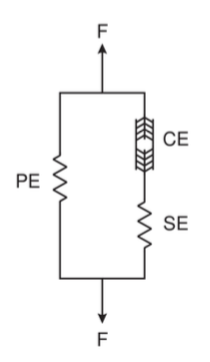
\includegraphics[scale=0.4]{Images/Hill.png}
		\caption{Schématisation du mucle par A.V. Hill \cite{berranen_simulation_2015}.}
		\label{Hill}
\end{figure}
Le muscle tel que représenté par A.V. Hill est composé de trois éléments distincts placés comme dans la figure \ref{Hill}. Un élément dit contractile (CE) y est placé en série avec un ressort appelé élément élastique (SE) et en parallèle avec un troisième élément dit passif (PE). L'élément contractile représente les mécanisme à l'origine de la contraction, ceux-ci tiennent compte à la fois de la longueur, de la force et enfin de la vitesse, les trois variables rattachés aux fonctions musculaires d'aprés A.V.Hill \cite{linden_mechanical_1998}. L'élément élastique quand à lui correspond aux tendons et aux aponévroses, ces tissus passifs élastiques on tendance à s'allonger durant un contraction isométrique. Enfin l'élément passif caractérise la résistance des tissus à l'élongation \cite{berranen_simulation_2015}.

La contraction est ainsi decrite par une equation reliant la longueur musculaire et la force ensendrée par le muscle présenté ci-dessous : 

% Equation ici !!!!!!!

Une autre equation permet quant à elle de relier la force et la vitesse de contraction : 

% Deuxième equation ici !!!!!

L'integration des deux équations précédentes conduit à l'expression du modèle mathématique de l'element contractile : 

% Troisième équation ici !!!! 


\section{Les modèle de Millard et thelen}

\section{Autres modèles}
Les modèles présentés plus haut ne sont pas les seuls a exister. En effet deux modèles peuvent notamment être mis en avant : le plus anciens datant de 1956 est le modèle de Huxley. Celui s'interesse au phénomènes biologiques etc ... \cite{huxley_muscle_1957}
\chapter{OpenSim : Un outil de simulation puissant et complet}

Présentation d'OpenSim 

Première aproche $\rightarrow$ les tutos

Review rapide du fonctionnement (diférents fichier etc ..) $\rightarrow$ peut être en annexe ? 
\chapter{Fournir un modèle musculaire à même de simuler la spasticité}
\section{La spasticité}
\section{Choisir un modèle}
Modèle de bas du corps (vs modèle de bras comme tristan ??)
\section{Adaptations du modèle}
à partir de ce que tristan avait fait 

plug in et resultats 
\chapter{Retours personnel}
Difficultés et compétences acquises 
Parler du passage de windows à mac et aussi de l'ancienne à la nouvelle version de openSim \\

Aprrendre a garder des traces claires et organisées de mon travail/ de mes recherches 